\begin{itemize}
    \item[الف)]
 ابعاد تصویر ورودی را برابر $(n_h, n_w, n_c)$ درنظر بگیرید. بر روی این ورودی یک لایه کانولوشن با فیلتر $1 \times 1$ با استراید و پدینگ استفاده می‌کنیم. کدام یک از عبارات زیر صحیح است؟ (تمام موارد صحیح را انتخاب کنید و کامل توضیح دهید.)
\newline
1. شما می‌توانید $n_c$ را با استفاده از کانولوشن $1 \times 1$ کاهش دهید. با این حال، نمی‌توانید $n_h, n_w$ را تغییر دهید.
\newline
2. شما می‌توانید از ماکس پولینگ استاندارد فقط برای کاهش $n_h, n_w$ و نه $n_c$ استفاده کنید.
\newline
3. شما می‌توانید از کانولوشن $1 \times 1$ برای کاهش $n_h, n_w, n_c$ استفاده کنید.
\newline
4. شما می‌توانید از ماکس پولینگ برای کاهش $n_c$ استفاده کنید.
\newline
\newline

\item[ب)]
فرض کنید یک فیلتر $2 \times 2$ را با $stride=2$ روی یک تصویر $4 \times 4$ اعمال می‌کنیم. این عملیات کانولوشن را با ضرب یک ماتریس در بردار به صورت $Ax = z$ خلاصه کنید که در اینجا: $x$ همان تصویر اولیه و $z$ همان نقشه ویژگی پس از اعمال فیلتر خواهد بود.

\vspace{1cm}

\begin{center}
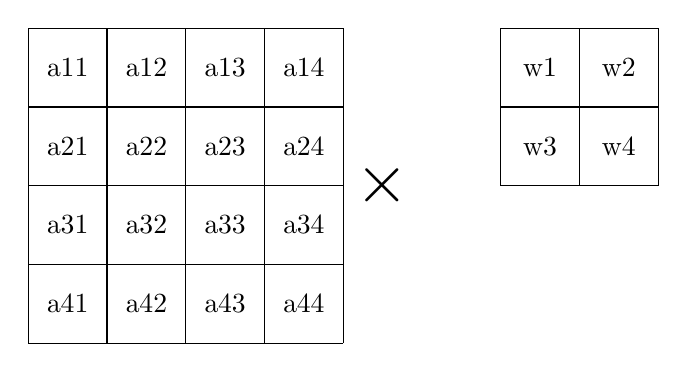
\begin{tikzpicture}
% Left grid
\draw[step=1cm] (0, 0) grid (4, 4);
\node at (0.5, 3.5) {a11};
\node at (1.5, 3.5) {a12};
\node at (2.5, 3.5) {a13};
\node at (3.5, 3.5) {a14};

\node at (0.5, 2.5) {a21};
\node at (1.5, 2.5) {a22};
\node at (2.5, 2.5) {a23};
\node at (3.5, 2.5) {a24};

\node at (0.5, 1.5) {a31};
\node at (1.5, 1.5) {a32};
\node at (2.5, 1.5) {a33};
\node at (3.5, 1.5) {a34};

\node at (0.5, 0.5) {a41};
\node at (1.5, 0.5) {a42};
\node at (2.5, 0.5) {a43};
\node at (3.5, 0.5) {a44};

% Right grid
\draw[step=1cm] (6, 2) grid (8, 4);
\node at (6.5, 3.5) {w1};
\node at (7.5, 3.5) {w2};
\node at (6.5, 2.5) {w3};
\node at (7.5, 2.5) {w4};

% Multiplication symbol
\node at (4.5, 2) {\Huge $\times$};

\end{tikzpicture}
\end{center}
\end{itemize}